\section*{Призма}

\subsection*{Дисперсия показателя преломления}

Принцип действия призмы основан на зависимости коэффициента преломления стекла от длины световой волны. Зная характеристики стекла, а именно показатели преломления для голубой($n_{1}$) и красной($n_{2}$) линий можно определить одну из основных характеристик спектрального прибора: дисперсию показателя преломления: 

\begin{center}
	{\Large $\frac{dn}{d\lambda} \approx \frac{n_{1} - n_{2}}{\lambda_{1} - \lambda_{2}}$}
\end{center}
	
Оценим угол $\delta\phi$ между волновыми фронтами двух близких линий $\lambda$ и $\lambda + \delta\lambda$. Пусть на призму с основанием a падает параллельный пучок света шириной $h$, и этот пучок целиком заполняет призму. Показанный на рис. 1 симметричный ход лучей (внутри призмы лучи распространяются параллельно основанию) соответствует углу наименьшего отклонения падающего пучка $\theta$, который в свою очередь зависит от преломляющего угла призмы $\alpha$ и показателя преломления $n(\lambda)$.

\begin{figure}[H]
	\centering
	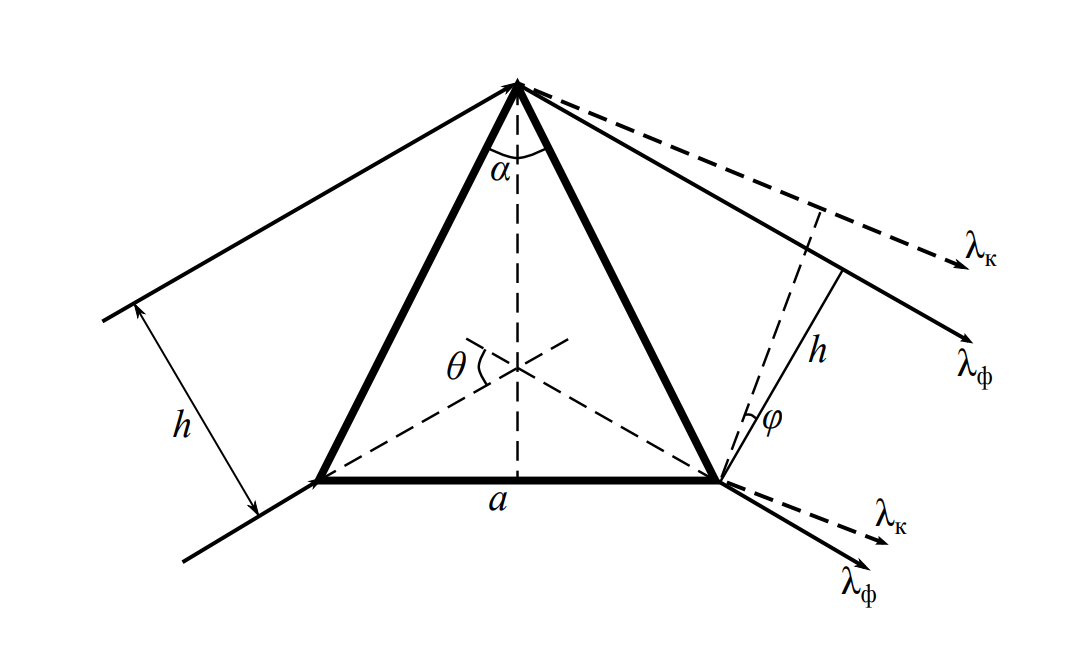
\includegraphics[width=0.4\textwidth]{../Изображения/Ход лучей для наименьшего отклонения.png}
	\caption{Ход лучей для наименьшего отклонения}
\end{figure}

Максимальная разность хода двух лучей с длиной волны $\lambda$ и $\lambda + \delta \lambda$ возникает вблизи основания призмы:

\begin{center}
	{\Large $\Delta = a[n(\lambda + \delta\lambda) - n(\lambda))] \approx a\frac{dn}{d\lambda}\delta\lambda = h\delta\phi$}
\end{center}

Типичная зависимость $n(\lambda)$, или закон дисперсии показателя преломления, приведена на рис.2. В области, закрашенной серым, показатель преломления растёт с длиной волны $dn/d\lambda > 0$ — это так называемая область \textit{аномальной дисперсии}. \textit{Аномальная дисперсия} имеет место на частотах, близких к резонансным, и соответственно в этой области велико поглощение света. В области, далёкой от резонансов, вещество прозрачно, а показатель преломления убывает с ростом длины волны, $dn/d\lambda < 0$, — это область нормальной дисперсии. Стекло в оптическом диапазоне длин волн имеет нормальную дисперсию (аномальная дисперсия в стекле имеет место в ультрафиолетовой области спектра).

\begin{figure}[H]
	\centering
	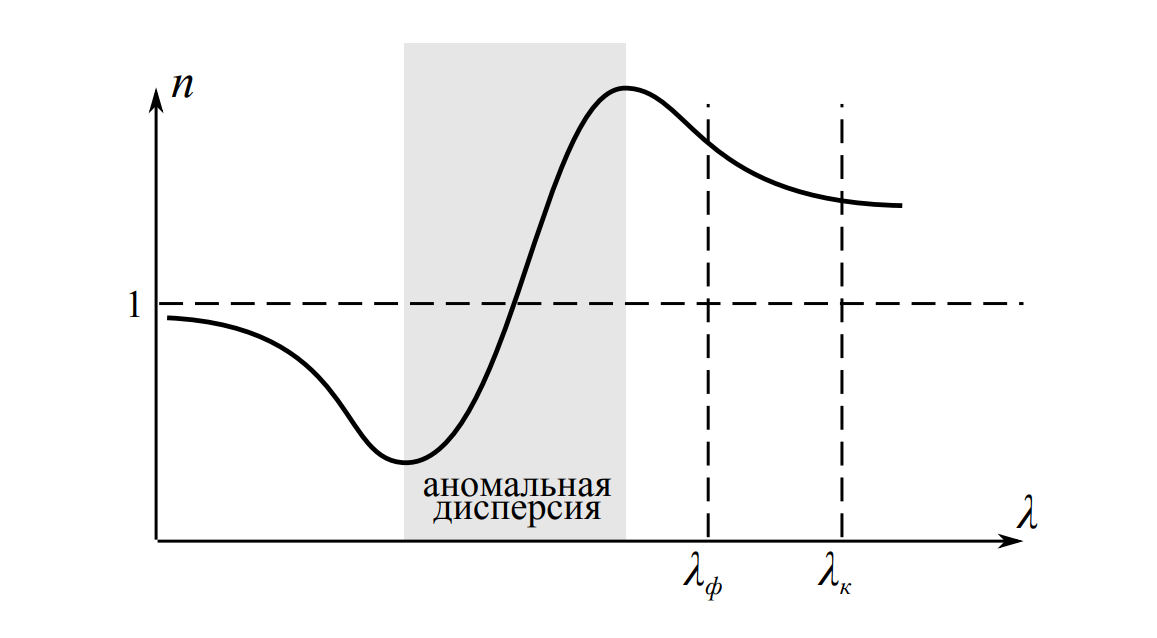
\includegraphics[width=0.6\textwidth]{../Изображения/Зависимость показателя преломления стекла от длины волны.png}
	\caption{Зависимость показателя преломления стекла от длины волны}
\end{figure}

\subsection*{Угловая дисперсия}

Угловая дисперсия $D(\lambda)$ характеризует угловое расстояние между
близкими спектральными линиями:

\begin{center}
	{\Large $D(\lambda) = \frac{d\phi}{d\lambda}$}
\end{center}

В современных приборах спектроскопии регистрация изображения спектров проводится не глазом, а линейкой или матрицей чувствительных к свету элементов. Угловая дисперсия позволяет определить минимальное расстояние между ячейками приёмного устройства: если требуется разрешить две спектральные линии с разностью длин волн $\delta\lambda$, то расстояние между элементами приемного устройства должно быть заметно меньше $D\delta\lambda f$, где f — фокусное расстояние объектива зрительной трубы.

В случае призмы из уравнения максимальной разности хода следует:
\begin{center}
	{\Large $D(\lambda) = \frac{d\phi}{d\lambda} = \frac{a}{h} \frac{dn}{d\lambda}$}
\end{center}

\subsection*{Показатель преломления}
Показатель преломления материала призмы $n(\lambda)$ удобно определять по углу наименьшего отклонения $\delta(\lambda)$ (рис.1). Минимальное отклонение луча, преломлённого призмой, от направления луча, падающего на призму, получается при симметричном ходе луча (в призме луч идёт параллельно основанию). Угол минимального отклонения $\delta$, преломляющий угол $/alpha$ и показатель преломления связаны соотношением:

\begin{center}
	{\Large $n(\lambda) = \frac{\sin\frac{\alpha + \delta(\lambda))}{2}}{sin\frac{\alpha}{2}}$}
\end{center}





